\subsubsection{AStar (A\*)}\label{sec:astar}
The A* Algorithms is a powerful algorithm used in many games (\cite{cai_2015_a}). Like UCS the algorithm uses weighted graph. The A* algorithm is faster than UCS and this is due to a heuristic value that takes notice of the location in relation to the end goal. This heuristic is they key difference between UCS and A* as having this allows A* to select the next node with the lowest cost AND closest to the goal as opposed to just the lowest cost (\cite{cai_2015_a}). For this reason, A* will navigate towards the goal as opposed to spanning out from the start point, this in turn leads to A* being the fastest algorithm on this list. Figure \ref{fig:dijkvsastar} contains a comparison of A* vs Dijkstra, this figure re-enforces research and the results found. However, it's also worth noting the implementation of the Dijkstra's algorithm from this source is closer to UCS than to standard Dijkstra. 
\begin{figure}[h]
	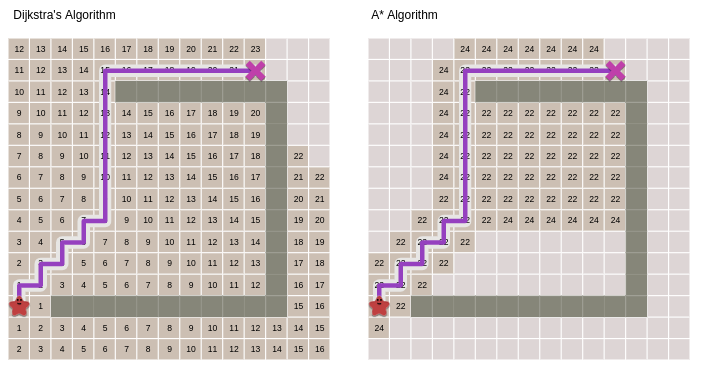
\includegraphics[width=\linewidth]{images/research/Dijkstrasvastar.png}\\
	\caption{Visual comparison Dijkstras(Adapted) vs A* generated from (\cite{redblobgames_2014_red})}
	\label{fig:dijkvsastar}
\end{figure}
